%%%%%%%%%%%%%%%%%%%%%%%%%%%%%%%%%%%%%%%%%
% This is an __unofficial__  LaTeX template  for project reports in SZU.
% This template is a modification based LaTeX template downloaded 
% from http://www.latextemplates.com

%%%%%%%%%%%%%%%%%%%%%%%%%%%%%%%%%%%%%%%%%

%----------------------------------------------------------------------------------------
%	PACKAGES AND OTHER DOCUMENT CONFIGURATIONS
%----------------------------------------------------------------------------------------

\documentclass{article}

\usepackage{fancyhdr} % Required for custom headers
\usepackage{lastpage} % Required to determine the last page for the footer
\usepackage{extramarks} % Required for headers and footers
\usepackage[usenames,dvipsnames]{color} % Required for custom colors
\usepackage{graphicx} % Required to insert images
\usepackage{listings} % Required for insertion of code
%\usepackage{courier} % Required for the courier font
\usepackage{lipsum} % Used for inserting dummy 'Lorem ipsum' text into the template
\usepackage{xcolor}
\usepackage{hyperref}
\usepackage{indentfirst}
\usepackage[BoldFont,SlantFont,CJKsetspaces,CJKchecksingle]{xeCJK}
\setCJKmainfont[BoldFont=SimHei]{SimSun}
\setCJKmonofont{SimSun}% 设置缺省中文字体
\parindent 2em   %段首缩进
\hypersetup{
    bookmarks=true,         % show bookmarks bar?
    unicode=false,          % non-Latin characters in Acrobat’s bookmarks
    pdftoolbar=true,        % show Acrobat’s toolbar?
    pdfmenubar=true,        % show Acrobat’s menu?
    pdffitwindow=false,     % window fit to page when opened
    pdfstartview={FitH},    % fits the width of the page to the window
    pdftitle={My title},    % title
    pdfauthor={Author},     % author
    pdfsubject={Subject},   % subject of the document
    pdfcreator={Creator},   % creator of the document
    pdfproducer={Producer}, % producer of the document
    pdfkeywords={keyword1} {key2} {key3}, % list of keywords
    pdfnewwindow=true,      % links in new window
    colorlinks=true,       % false: boxed links; true: colored links
    linkcolor=red,          % color of internal links (change box color with linkbordercolor)
    citecolor=green,        % color of links to bibliography
    filecolor=magenta,      % color of file links
    urlcolor=cyan           % color of external links
}

% Margins
\topmargin=-0.45in
\evensidemargin=0in
\oddsidemargin=0in
\textwidth=6.5in
\textheight=9.0in
\headsep=0.25in

\linespread{1.1} % Line spacing

% Set up the header and footer
\pagestyle{fancy}
%\lhead{\hmwkAuthorName} % Top left header
\chead{\hmwkClass\ \hmwkTitle} % Top center head
\rhead{\firstxmark} % Top right header
\lfoot{\lastxmark} % Bottom left footer
\cfoot{} % Bottom center footer
\rfoot{Page\ \thepage\ of\ \protect\pageref{LastPage}} % Bottom right footer
\renewcommand\headrulewidth{0.4pt} % Size of the header rule
\renewcommand\footrulewidth{0.4pt} % Size of the footer rule

\setlength\parindent{0pt} % Removes all indentation from paragraphs

%----------------------------------------------------------------------------------------
%	CODE INCLUSION CONFIGURATION
%----------------------------------------------------------------------------------------

\definecolor{MyDarkGreen}{rgb}{0.0,0.4,0.0} % This is the color used for comments
\lstloadlanguages{Perl} % Load Perl syntax for listings, for a list of other languages supported see: ftp://ftp.tex.ac.uk/tex-archive/macros/latex/contrib/listings/listings.pdf
\lstset{numbers=left,
numberstyle=\tiny,
keywordstyle=\color{blue!70}, commentstyle=\color{red!50!green!50!blue!50},
frame=shadowbox,
rulesepcolor=\color{red!20!green!20!blue!20}
}

% Creates a new command to include a perl script, the first parameter is the filename of the script (without .pl), the second parameter is the caption
\newcommand{\perlscript}[2]{
\begin{itemize}
\item[]\lstinputlisting[caption=#2,label=#1]{#1.pl}
\end{itemize}
}

%----------------------------------------------------------------------------------------
%	DOCUMENT STRUCTURE COMMANDS
%	Skip this unless you know what you're doing
%----------------------------------------------------------------------------------------

% Header and footer for when a page split occurs within a problem environment
\newcommand{\enterProblemHeader}[1]{
\nobreak\extramarks{#1}{#1 接下页\ldots}\nobreak
\nobreak\extramarks{#1 (续)}{#1 接下页\ldots}\nobreak
}

% Header and footer for when a page split occurs between problem environments
\newcommand{\exitProblemHeader}[1]{
\nobreak\extramarks{#1 (续)}{#1 接下页\ldots}\nobreak
\nobreak\extramarks{#1}{}\nobreak
}

\setcounter{secnumdepth}{0} % Removes default section numbers
\newcounter{homeworkProblemCounter} % Creates a counter to keep track of the number of problems

\newcommand{\homeworkProblemName}{}
\newenvironment{homeworkProblem}[1][Problem \arabic{homeworkProblemCounter}]{ % Makes a new environment called homeworkProblem which takes 1 argument (custom name) but the default is "Problem #"
\stepcounter{homeworkProblemCounter} % Increase counter for number of problems
\renewcommand{\homeworkProblemName}{#1} % Assign \homeworkProblemName the name of the problem
\section{\homeworkProblemName} % Make a section in the document with the custom problem count
\enterProblemHeader{\homeworkProblemName} % Header and footer within the environment
}{
\exitProblemHeader{\homeworkProblemName} % Header and footer after the environment
}

\newcommand{\problemAnswer}[1]{ % Defines the problem answer command with the content as the only argument
\noindent\framebox[\columnwidth][c]{\begin{minipage}{0.98\columnwidth}#1\end{minipage}} % Makes the box around the problem answer and puts the content inside
}

\newcommand{\homeworkSectionName}{}
\newenvironment{homeworkSection}[1]{ % New environment for sections within homework problems, takes 1 argument - the name of the section
\renewcommand{\homeworkSectionName}{#1} % Assign \homeworkSectionName to the name of the section from the environment argument
\subsection{\homeworkSectionName} % Make a subsection with the custom name of the subsection
\enterProblemHeader{\homeworkProblemName\ [\homeworkSectionName]} % Header and footer within the environment
}{
\enterProblemHeader{\homeworkProblemName} % Header and footer after the environment
}

%----------------------------------------------------------------------------------------
%	NAME AND CLASS SECTION
%----------------------------------------------------------------------------------------

\newcommand{\hmwkTitle}{进程控制和守护进程的创建} % Assignment title
\newcommand{\hmwkDueDate}{Monday,\ January\ 1,\ 2012} % Due date
\newcommand{\hmwkClass}{Linux系统编程} % Course/class
\newcommand{\hmwkClassTime}{10:30am} % Class/lecture time
\newcommand{\hmwkClassInstructor}{老师姓名} % Teacher/lecturer
\newcommand{\hmwkAuthorName}{报告人姓名} % Your name
\newcommand{\studentID}{2011XXXXXX}
\newcommand{\reportName}{深圳大学实验报告}
\newcommand{\collegeName}{计算机与软件学院}
\newcommand{\majors}{数学与应用数学,计算机科学与技术}
\newcommand{\labTime}{2014年3月24日}
\newcommand{\submitTime}{2014年4月25日}  

%----------------------------------------------------------------------------------------
%	TITLE PAGE
%----------------------------------------------------------------------------------------

\begin{document}
\begin{titlepage}

\title{\reportName}
\date{}
\maketitle

\begin{center}
\begin{large}
\begin{tabular}{cc}
课程名称:& \hmwkClass\\
\cline{2-2}\\
实验项目名称:& \hmwkTitle\\
\cline{2-2}\\
学\qquad 院:& \collegeName\\
\cline{2-2}\\
专\qquad 业:& \majors\\
\cline{2-2}\\
指导老师:& \hmwkClassInstructor \\
\cline{2-2}\\
学生姓名:& \hmwkAuthorName \\
\cline{2-2}\\
学\qquad 号:& \studentID \\
\cline{2-2} \\
实验时间:& \labTime \\
\cline{2-2} \\
报告提交时间:& \submitTime \\
\cline{2-2}
\end{tabular}
\end{large}
\end{center}
%\vfill \hfill
\end{titlepage}


%----------------------------------------------------------------------------------------

%\maketitle

%----------------------------------------------------------------------------------------
%	TABLE OF CONTENTS
%----------------------------------------------------------------------------------------

%\setcounter{tocdepth}{1} % Uncomment this line if you don't want subsections listed in the ToC

\newpage
\tableofcontents
\newpage

%----------------------------------------------------------------------------------------
%	SECTION 1
%----------------------------------------------------------------------------------------
\section{实验目标}

\begin{enumerate}
\item 掌握fork()系统调用及进程的相关概念
\item 掌握wait()和waitpid()系统调用
\item 掌握进程组,会话进程等概念和setsid()系统调用
\item 掌握文件重定向的技巧
\item 掌握创建守护进程的步骤及其实现
\end{enumerate}

%----------------------------------------------------------------------------------------
%	SECTION 2
%----------------------------------------------------------------------------------------
\section{实验环境与工件}

\begin{enumerate}
\item 湖边Linux实验室  
\item Fedora 13
\end{enumerate}

%----------------------------------------------------------------------------------------
%	SECTION 3
%----------------------------------------------------------------------------------------
\section{实验内容与步骤}

下面的程序会用到如下程序段:从命令行获取数字参数,参考实现见下图:
\begin{center}
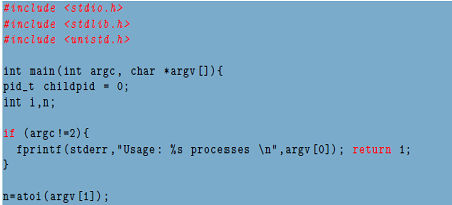
\includegraphics[width=0.75\columnwidth]{picture1} % Example image
\end{center}

%----------------------------------------------------------------------------------------
%	PROBLEM 1
%----------------------------------------------------------------------------------------
\subsection{问题一}
编例实现创建n个子进程P1,P2,…,Pn,其中,各进程之间的关系是:P1是调用进程的子进程,P(k+1)是Pk的子进程。请打印各进程本身的进程号、父进程号,子进程号。参考运行结果如下。要求:(1)每个父进程都要等待子进程退出后才能退出;(2)n通过命令行参数传入;(3)附上源代码截图和运行结果截图。(20分) \\

相关代码:

\begin{lstlisting}[language=C]
#include <stdio.h>
#include <stdlib.h>
#include <unistd.h>

int main(int argc, char *argv[]){
	pid_t child_pid = 0;
	int i, n;

	if (argc != 2){
		fprintf(stderr, "Usage: %s process \n", argv[0]);
		return 1;
	}

	n = atoi(argv[1]);

	for (i = 0; i < n; i++){
		child_pid = fork();
		if (child_pid > 0){
			printf("Process id: %d, parent id: %d ", \
			getpid(), getppid());
			printf("child id: %d\n", child_pid);
			break;
		} else if (child_pid < 0) {
			printf("fork error!\n");
			exit(-1);
		}
	}

	if (i == n){
		printf("Process id: %d, parent id: %d ", getpid(), getppid());
		printf("child_pid: %d\n", child_pid);
	}

	if (child_pid > 0){
		waitpid(child_pid, NULL, 0);
	}
	return 0;
}
\end{lstlisting}

实验结果:
\begin{center}
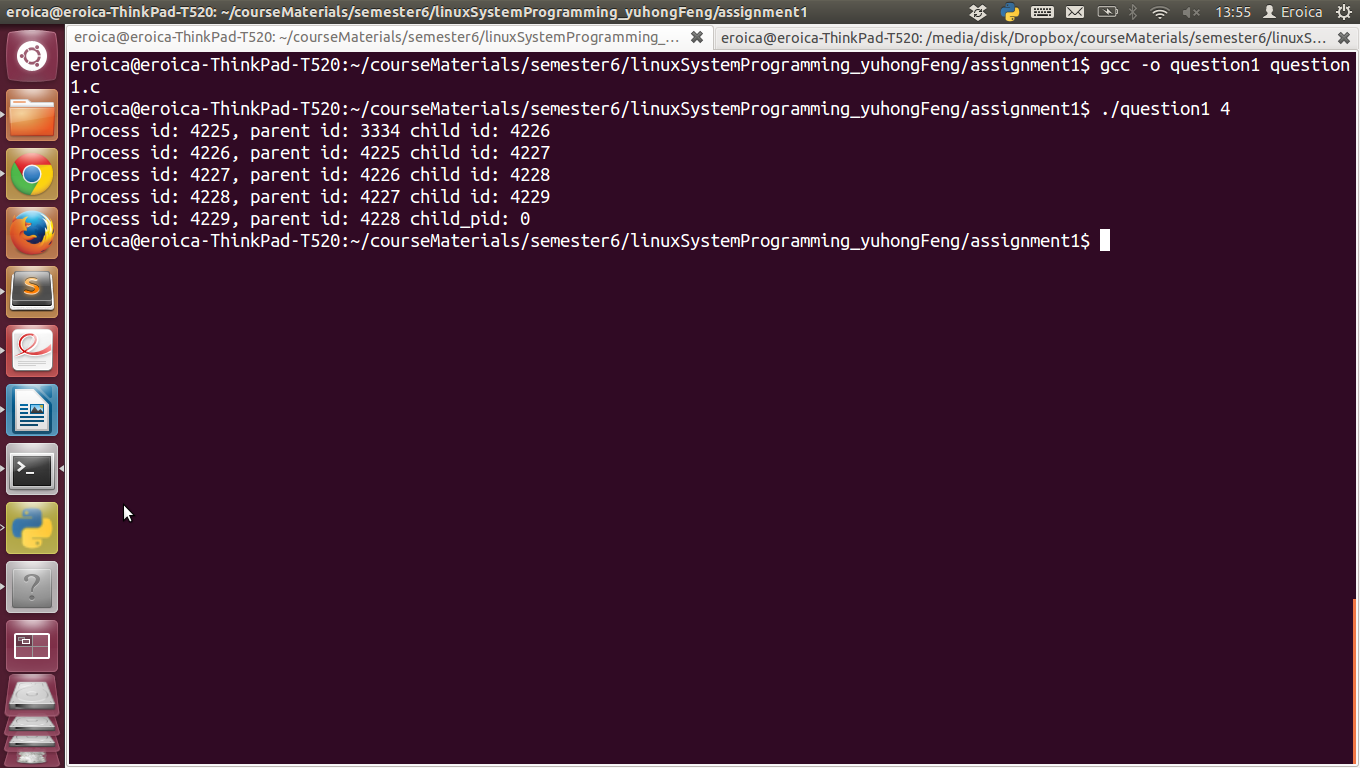
\includegraphics[width=0.8\columnwidth]{pic_question1} % Example image
\end{center}

%----------------------------------------------------------------------------------------
%	PROBLEM 2
%----------------------------------------------------------------------------------------
\subsection{问题二}
编例实现创建n个子进程P1,P2,…,Pn,其中,各进程之间的关系是:P1,…,Pn都是调用进程的子进程。请打印各进程本身的进程号、父进程号,子进程号。参考运行结果如下。要求:(1)每个父进程都要等待子进程退出后才能退出;(2)n通过命令行参数传入;(3)附上源代码截图和运行结果截图。(20分) \\

相关代码:

\begin{lstlisting}[language=C]
#include <stdio.h>
#include <stdlib.h>
#include <unistd.h>

int main(int argc, char *argv[]){
	pid_t child_pid = 0;
	int i, j, n;
	int child_IDS[200];

	if (argc != 2){
		fprintf(stderr, "Usage: %s process \n", argv[0]);
		return 1;
	}

	n = atoi(argv[1]);

	for (i = 0; i < n; i++){
		child_pid = fork();
		if (child_pid > 0){
			child_IDS[i] = child_pid;
		}
		if (child_pid == 0){
			printf("Process ID: %d, parent ID: %d ", \
			getpid(), getppid());
			printf("child ID: %d\n", child_pid);
			exit(1);
		} else if (child_pid < 0) {
			printf("fork error!\n");
			exit(-1);
		}
	}

	if (child_pid > 0){
		waitpid(child_pid, NULL, 0);
	}

	if (i == n){
		printf("process ID: %d, child IDs:", getpid());
		for (j = 0; j < n; j++){
			printf("%d ", child_IDS[j]);
		}
		printf("\n");
	}

	return 0;
}
\end{lstlisting}

实验结果:

\begin{center}
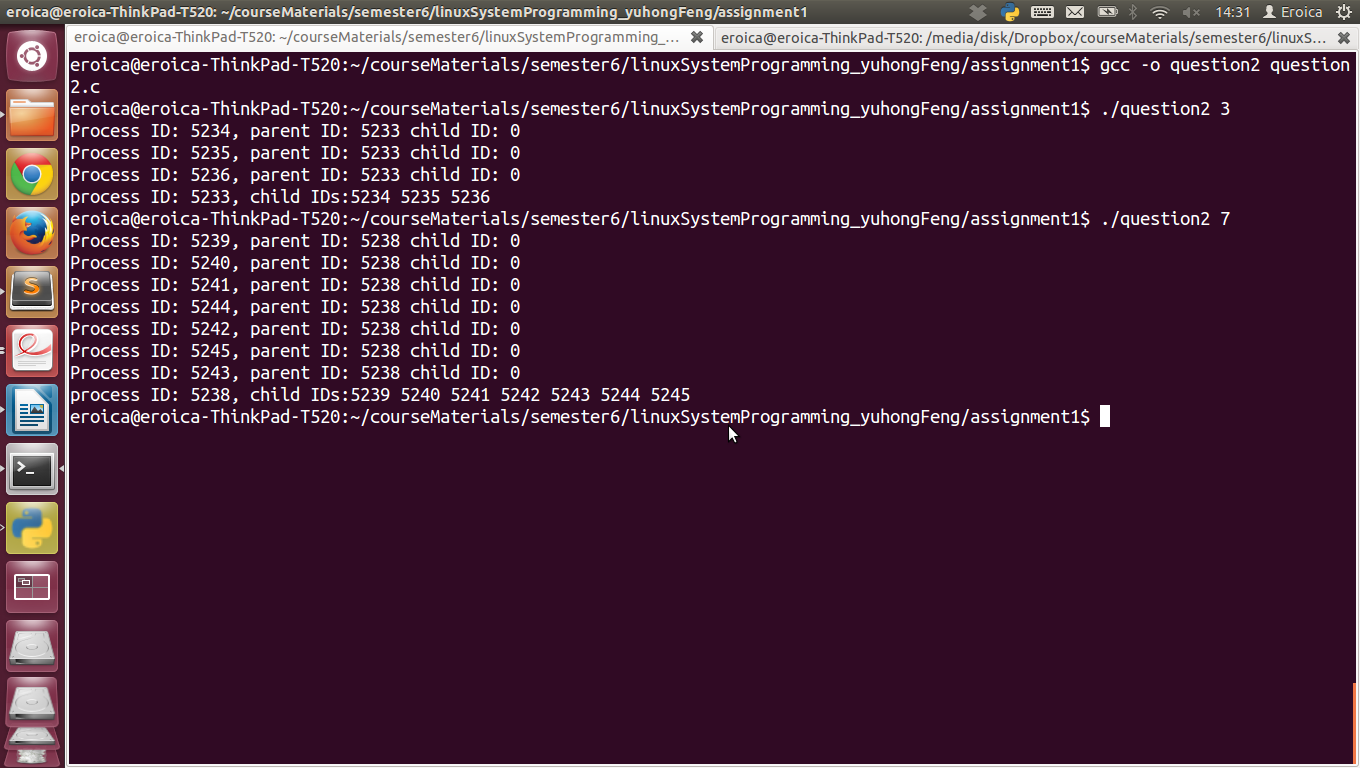
\includegraphics[width=0.8\columnwidth]{pic_question2} % Example image
\end{center}


\end{document}
